\documentclass[titlepage]{article}
\usepackage[bottom=3cm, right=3cm, left=3cm, top=3cm]{geometry}
\usepackage {graphicx}
\usepackage{caption}
%opening
\title{%
	Practical Machine Learning\\
	
	\vspace*{2em}
	\LARGE Exercise 3 \\
	Spring 2024}
\author{Lisa Stafford}
\date{February 20, 2024}

\begin{document}
	\setlength\parindent{0pt}
	
	\maketitle
	
	\section*{Abstract}
	Model selection is a common problem for machine learning architects where one selects the model that does the best job of generalizing and most appropriate for the given problem.  Those selecting the model should choose the best balance between under- and over-fitting.  When selecting a model, one must examine the value of different predictive methods to identify the one that best fits observable data.  There are two main factors when choosing the most appropriate model in machine learning.  One is the reason for choosing it, and the other is the model's performance.  Reasons for choosing a model should be based on the available data set, and the problem task.
	
	\section*{Introduction}
	In order to learn and determine which models are most effective, we used a wine data set obtained from the University of Irvine \cite{dataset}. Training is performed on each subset of red and white wine within the data set.  Several models are trained implementing libraries directly from scikitlearn \cite{scikitlearn} and then training and testing performance scores for each model and wine subsets are taken.  Model selection determinations can then be made based on the performance scores.  

	
	\section*{Dataset Description}
	Our Wine Dataset is actually comprised of two different wine subsets of data.  While both are related to variants of \cite{dataset} "Portuguese Vhinho Verde wine" the data is actually split in two subsets - one red subset and one white subset.  Each subset contains 11 features and 1 label for wine quality.   All features are continuous float values.  Within the model the "wine quality" labels are recognized as discrete categorical integer values ranging from 3 to 9 for the white wines, and 3 and 8 for the red wines.  White wine contains a total of 4898 total data instances, while red wine has a total of 1598 data instances as shown in the following table images. Figure 1 (left) displays feature values, statistics, and total instances for white wine, while Figure 1 (right) displays feature values, statistics and total instances available for red wine.
	
	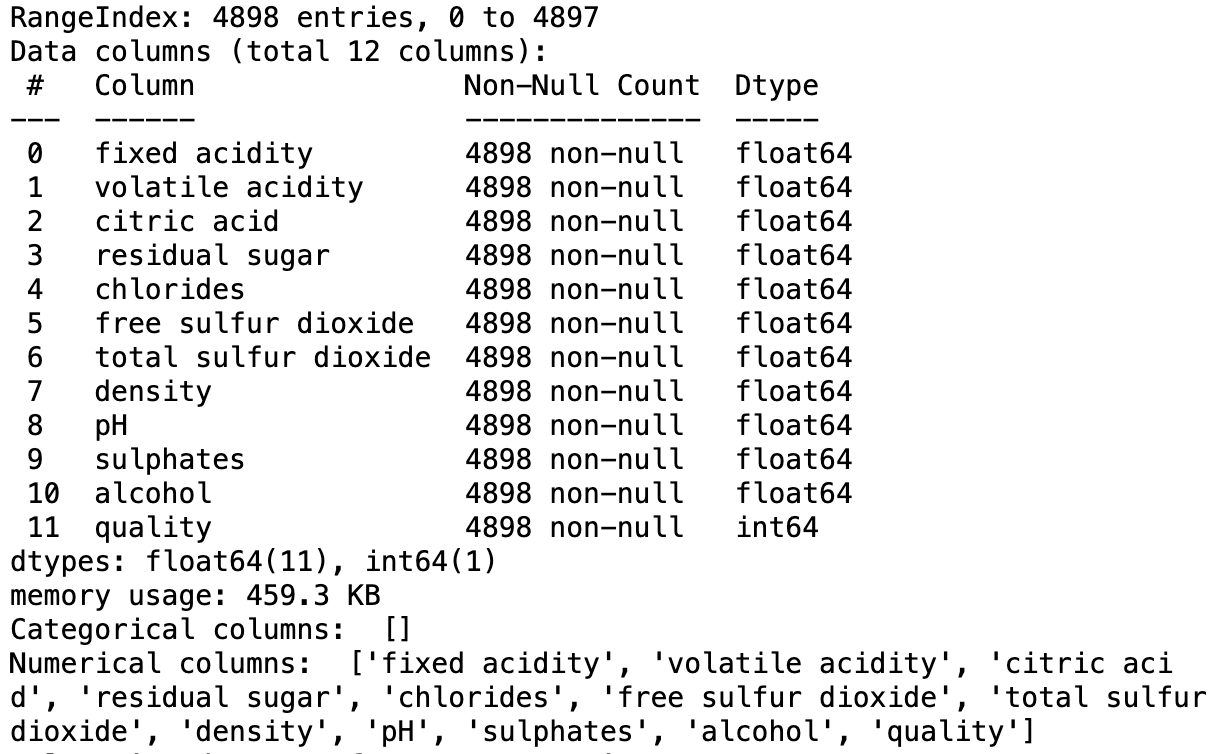
\includegraphics[width=.45\textwidth]{img/white.png}
	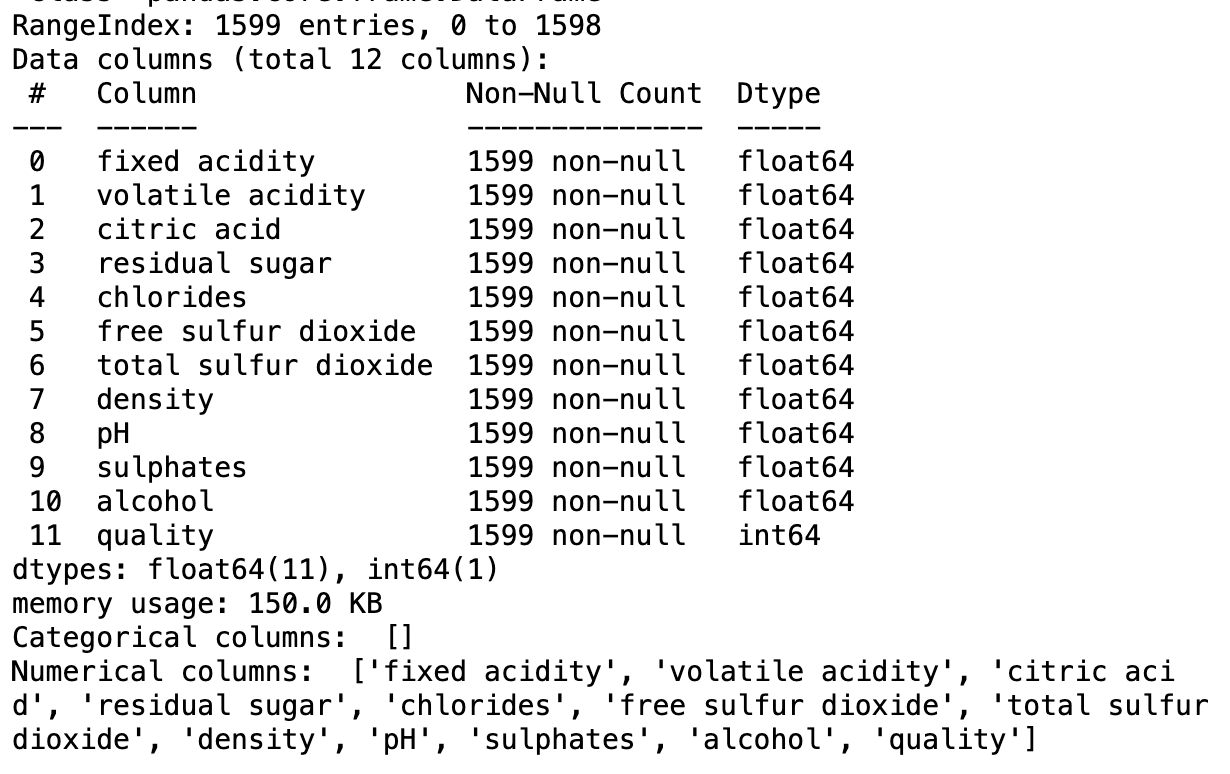
\includegraphics[width=.45\textwidth]{img/red.png}
	
	\noindent Data for both red and white wine datasets is somewhat "pre-cleaned".   The feature values are all continuous and both red and white datasets contain no missing data values.  However it should be noted that these features are not evenly distributed.  The data values are somewhat bell-shaped with a larger number of data instances with labels closer to the mean.  As described on the dataset website \cite{dataset} both "dataset... classes are ordered and []unbalanced] so there are many more normal wines than excellent or poor ones.... [also], both datasets have 11 physiochemical features... and a sensory output label, ('quality')".  Because Standard Scaling worked best as a data transformation method in Exercise 2, we use the same code to perform this specific data cleaning on the data again.  
	
	\section*{Experimental Setup}
	
		We are looking at the wine quality dataset, and trying to run a small number of machine learning algorithms on the dataset to determine the best machine learning algorithm for the dataset, where the "best" algorithm may be a set of algorithms.
		
		We know that this particular dataset is supervised and the problem is a classification problem with a known number of categories. Therefore we know that the best ML models will be in that realm.  To make an initial decision, this "cheat sheet" decision chart from sklearn \cite{scikitlearn} was followed: 
		
		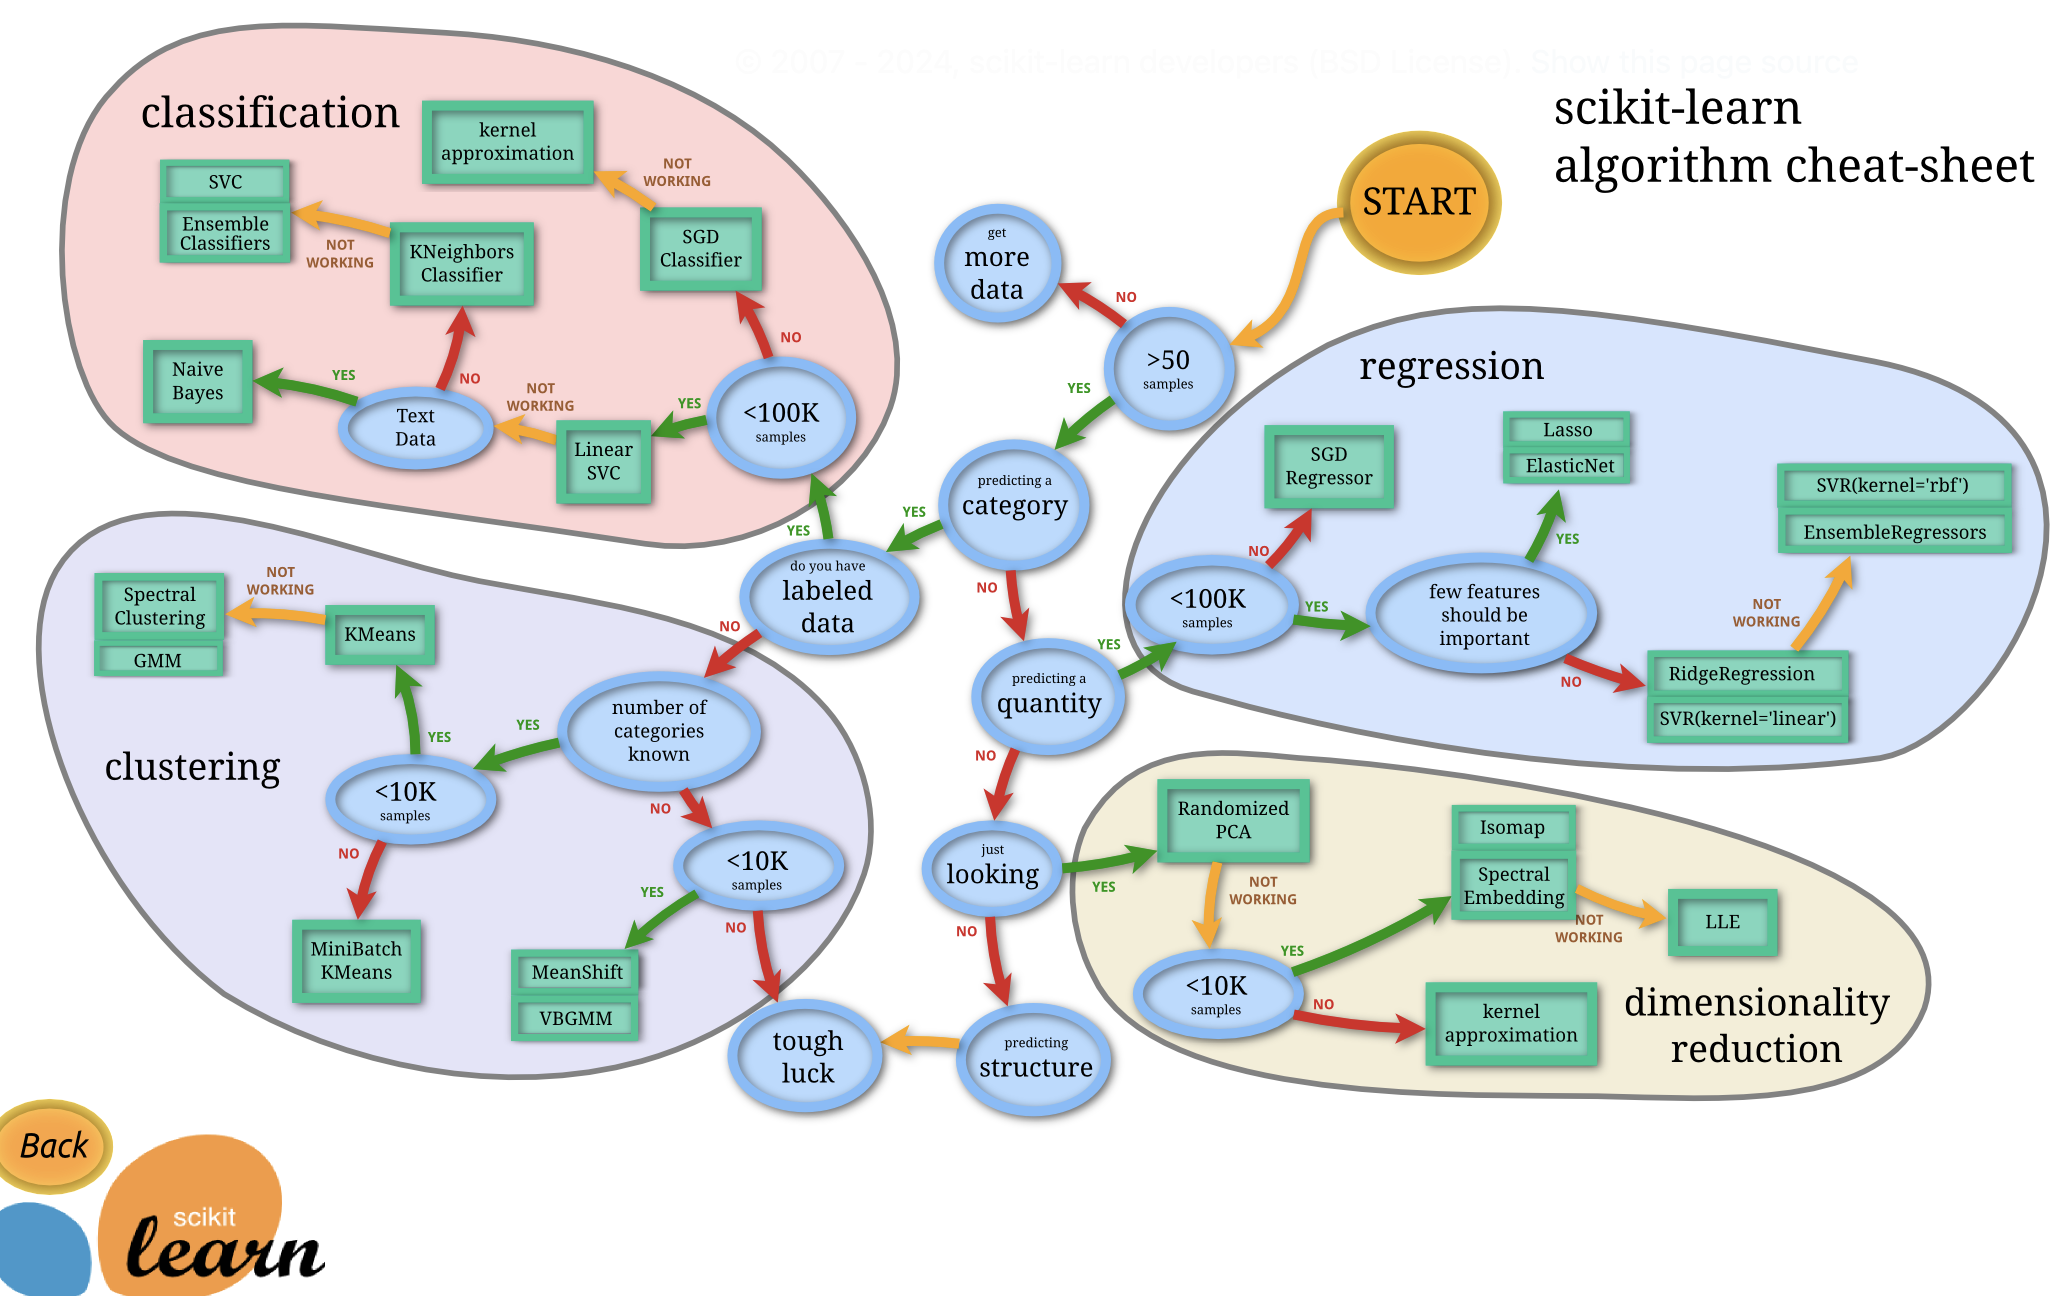
\includegraphics[width=.95\textwidth]{img/sklearncheatsheet.png}
		
		A decision was made to evaluate a number of popular Classification ML Models/Algorithms, since it was hard to be sure which would be more effective.  The machine learning algorithms that fit best with this particular dataset are as follows and therefore we will utilize these listed in our initial ML model selection:
	
	\begin{enumerate}
		\item Linear Support Vector Machine
		\item Classic Support Vector Machine
		\item K-Neighbors Classifier
		\item Stochastic Gradient Descent Classifier
		\item Neural Network using MultiLayer Perceptron
	\end{enumerate}
	
		While neural networks are not listed in the above decision chart, they are frequently used when training ML models due to their flexibility for use in a wide variety of ML problems, on different data types, and generally high level of performance. Therefore, they were included in this exercise.  Training is performed on each subset of red and white wine within the data set.  Several models are trained implementing libraries directly from scikitlearn \cite{scikitlearn}.  While we have a number of different model options, we specify limited hyper-parameters for each model, and instead frequently proceed with training using the default hyper-parameters specified through scikitlearn in most cases.  Next, training and testing performance scores for each model and wine subsets are taken.  Model selection determinations and evaluation is then to be made based on ten individual and unrelated train and test runs to get performance scores of each model.  Performance values are averaged after 10 independent model train/test runs.  
	 
	\section*{Results}
	Machine learning performance results were never very highly performative, but resulted as follows.  The highest machine learning test performance was found to be different models, depending on the wine subset.  
	\begin{center}
		 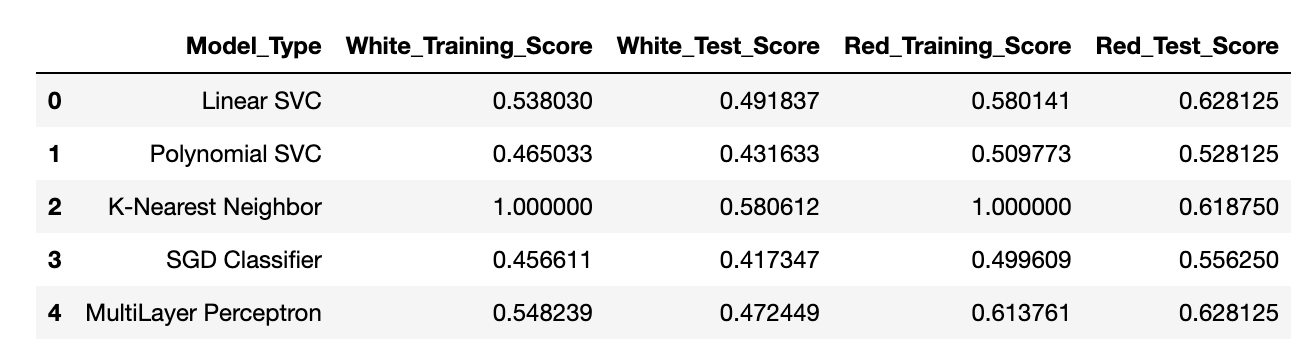
\includegraphics[width=.5\textwidth]{img/results.png}
	\end{center}
	
As shown in the chart, highest performance for the white wine subset was obtained using K-Nearest Neighbor achieving 58\% accuracy for performance on test data.  The red wine data subset resulted in the same performance for both Linear Support Vector Machine and NN using a Multi Layer Perceptron with 62.8\% accuracy for performance on test data.
	
	
\begin{thebibliography}{9}
	\bibitem{dataset1} A. Asuncion, D. Newman, UCI Machine Learning Repository, University of California, Irvine  (2007).  Obtained from https://archive-beta.ics.uci.edu/dataset/186/wine+quality. 
	\bibitem{numpyisnan} C. Harris, K. Millman, S. van der Walt,  Array programming with NumPy. Nature 585, 357–362 (2020). DOI: 10.1038/s41586-020-2649-2.  https://numpy.org/doc/stable/reference/generated/numpy.isnan.html
	\bibitem{seaborn} M. Waskom, (2021). seaborn: statistical data visualization. Journal of Open Source Software, 6(60), 3021, https://doi.org/10.21105/joss.03021.
	\bibitem{scikitlearn}Scikit-learn: Machine Learning in Python, Pedregosa et al., JMLR 12, pp. 2825-2830, 2011. 
\end{thebibliography}

\end{document}
